\title{Palette: Image-to-Image Diffusion Models}

\begin{abstract}
This paper develops a unified framework for image-to-image translation based on conditional diffusion models and evaluates this framework on four challenging image-to-image translation tasks, namely colorization, inpainting, uncropping, and JPEG restoration. Our simple implementation of image-to-image diffusion models outperforms strong GAN and regression baselines on all tasks, without task-specific hyper-parameter tuning, architecture customization, or any auxiliary loss or sophisticated new techniques needed. We uncover the impact of an L2 vs. L1 loss in the denoising diffusion objective on sample diversity, and demonstrate the importance of self-attention in the neural architecture through empirical studies. Importantly, we advocate a unified evaluation protocol based on ImageNet, with human evaluation and sample quality scores (FID, Inception Score, Classification Accuracy of a pre-trained ResNet-50, and Perceptual Distance against original images). We expect this standardized evaluation protocol to play a role in advancing image-to-image translation research. Finally, we show that a generalist, multi-task diffusion model performs as well or better than task-specific specialist counterparts. Check out \href{https://diffusion-palette.github.io/}{https://diffusion-palette.github.io/} for an overview of the results and code.
\end{abstract}

\section{Introduction}
\label{sec:intro}

Many problems in vision and image processing can be formulated as image-to-image translation. Examples include restoration tasks, like super-resolution, colorization, and inpainting, as well as pixel-level image understanding tasks, such as instance segmentation and depth estimation.  

Many such tasks, like those in Fig.\ \ref{fig:1}, are complex inverse problems, where multiple output images are consistent with a single input. A natural approach to image-to-image translation is to learn the conditional distribution of output images given the input, using deep generative models that can capture multi-modal distributions in the high-dimensional space of images.

Generative Adversarial Networks (GANs) \citep{goodfellow2014generative,radford2015unsupervised} have emerged as the model family of choice for many image-to-image tasks \citep{isola-cvpr-2017}; they are capable of generating high fidelity outputs, are broadly applicable, and support efficient sampling. Nevertheless, GANs can be challenging to train \cite{arjovsky-arxiv-2017,gulrajani2017improved}, and often drop modes in the output distribution~\cite{metz2016unrolled,ravuri2019classification}. Autoregressive Models \citep{oord2016conditional,parmar2018image}, VAEs \citep{Kingma2013,vahdat2021nvae}, and Normalizing Flows \citep{dinh2016density,Kingma2018} have seen success in specific applications, but arguably, have not established the same level of quality and generality as GANs.  

Diffusion and score-based models \citep{sohl2015deep,song-arxiv-2020,ho2020denoising} have received a surge of recent interest~\cite{cai-eccv-2020,song-iclr-2021,hoogeboom2021argmax,vahdat2021score,kingma2021variational,austin2021structured}, resulting in several key advances in modeling continuous data. On speech synthesis, diffusion models have achieved human evaluation scores on par with SoTA autoregressive models~\citep{chen-iclr-2021,chen-interspeech-2021,kong-arxiv-2020}. On the class-conditional ImageNet generation challenge they have outperformed strong GAN baselines in terms of FID scores~\citep{dhariwal2021diffusion,ho-arxiv-2021}. On image super-resolution, they have delivered impressive face enhancement results, outperforming GANs~\citep{saharia2021image}. Despite these results, it is not clear whether diffusion models rival GANs in offering a versatile and general framework for image manipulation.

This paper investigates the general applicability of {\em Palette}, our implementation of image-to-image diffusion models, to a suite of  distinct and challenging tasks, namely colorization, inpainting, uncropping, and JPEG restoration (see Figs.\ \ref{fig:1}, \ref{fig:panormauncrop}).
We show that Palette, with no task-specific architecture customization, nor changes to hyper-parameters or the loss,  delivers high-fidelity outputs across all four tasks. It outperforms task-specific baselines and a strong regression baseline with an identical neural architecture.

Importantly, we show that a single {\em generalist} Palette model, trained on colorization, inpainting and JPEG restoration, outperforms a task-specific JPEG model and achieves competitive performance on the other tasks.

We study key components of Palette, including the denoising loss function and the neural net architecture. We find that while $L_2$~\citep{ho2020denoising} and $L_1$~\citep{chen-iclr-2021} losses in the denoising objective yield similar sample-quality scores, $L_2$ leads to a higher degree of diversity in model samples, whereas $L_1$~\citep{chen-iclr-2021} produces more conservative outputs. We also find that removing self-attention layers from the U-Net architecture of Palette, to build a fully convolutional model, hurts performance. Finally, we advocate a standardized evaluation protocol for inpainting, uncropping, and JPEG restoration based on ImageNet~\citep{deng2009imagenet}, and we report sample quality scores for several baselines. We hope this benchmark will help advance image-to-image translation research.

\section{Related work}

Our work is inspired by Pix2Pix \citep{isola-cvpr-2017}, which explored myriad image-to-image translation tasks with GANs. GAN-based techniques have also been proposed for image-to-image problems like unpaired translation \citep{zhu2017unpaired}, unsupervised cross-domain generation \citep{taigman2016unsupervised}, multi-domain translation \citep{choi2018stargan}, and few shot translation \citep{liu2019few}. Nevertheless, existing GAN models are sometimes unsuccessful in holistically translating images with consistent structural and textural regularity.

Diffusion models  \citep{sohl2015deep} recently emerged with impressive results on image generation~\citep{ho2020denoising, ho-arxiv-2021, dhariwal2021diffusion}, audio synthesis~\citep{chen-iclr-2021, kong2020diffwave}, and image super-resolution~\citep{saharia2021image,Kadkhodaie2021}, as well as unpaired image-to-image translation~\citep{sasaki2021unit} and image editing~\citep{meng2021sdedit,sinha2021d2c}. Our conditional diffusion models build on these recent advances, showing versatility on a suite of image-to-image translation tasks.

Most diffusion models for inpainting and other linear inverse problems have adapted unconditional models for use in conditional tasks \cite{sohl2015deep,song-iclr-2021,meng2021sdedit}.

This has the advantage that only one model need be trained.  However, unconditional tasks are often more difficult than conditional tasks. We cast Palette as a conditional model, opting for multitask training should one want a single model for multiple tasks.

Early \textbf{inpainting} approaches 

\cite{bertalmio2000image, barnes2009PAR, he2012statistics,hays2007scene}

work well on textured regions but often fall short in generating semantically consistent structure. GANs are widely used but often require auxiliary objectives on structures, context, edges, contours and hand-engineered features~\cite{iizuka2017globally, yu2018generative, yu2019free,nazeri2019edgeconnect, yi2020contextual, liu2020rethinking, kim2021zoomtoinpaint}, and they lack diversity in their outputs  \citep{zheng2019pluralistic, zhao2021large}.

\textbf{Image uncropping} (a.k.a.\ outpainting) is considered more challenging than inpainting as it entails generating open-ended content with less context. Early methods relied on retrieval \citep{kopf2012quality, wang2014biggerpicture, shan2014uncrop}. GAN-based methods are now predominant  \cite{teterwak2019boundless}, but are often domain-specific \cite{yang2019very, bowen2021oconet,wang2019srn, cheng2021out, lin2021infinitygan}. We show that conditional diffusion models trained on large  datasets reliably address both inpainting and uncropping across image domains.

{\bf Colorization} is a well-studied

task \cite{coltran,guadarrama2017pixcolor,royer-arxiv-2017,ardizzone-arxiv-2017}, requiring a degree of scene understanding, which makes it a natural choice for self-supervised learning~\citep{larsson2016learning}. Challenges include diverse colorization~\citep{deshpande2017learning}, respecting semantic categories~\citep{zhang2016colorful}, and producing high-fidelity color~\cite{guadarrama2017pixcolor}. While some prior work makes use of specialized auxiliary classification losses, we find that generic image-to-image diffusion models work well  without task-specific specialization.
\textbf{JPEG restoration} (aka. JPEG artifact removal) is the nonlinear inverse problem of removing compression artifacts. \cite{dong2015compression} applied deep CNN architectures for JPEG restoration, and \cite{galteri2017deep, galteri2019deep} successfully applied GANs  for artifact removal, but they have been restricted to quality factors above 10. We show the effectiveness of Palette in removing compression artifacts for quality factors as low as 5. 

{\bf Multi-task training} is a relatively under-explored area in image-to-image translation.
\citep{guocheng2019trinity, yu2018crafting} train simultaneously on multiple  tasks, but they focus primarily on enhancement tasks like deblurring, denoising, and super-resolution, and they use smaller modular networks. Several works have also dealt with simultaneous training over multiple degradations on a single task e.g. multi-scale super-resolution \citep{kim2016deeply}, and JPEG restoration on multiple quality factors \citep{galteri2019deep, liu2018multi}. With Palette we take a first step toward building multi-task image-to-image diffusion models for a wide variety of tasks.

\section{Palette}

Diffusion models \citep{sohl2015deep,ho2020denoising} convert samples from a standard Gaussian distribution into samples from an empirical data distribution through an iterative denoising process. Conditional diffusion models \citep{chen-iclr-2021,saharia2021image} make the denoising process conditional on an input signal. Image-to-image diffusion models are conditional diffusion models of the form $p({\bm{y}} \mid {\bm{x}})$, where both ${\bm{x}}$ and ${\bm{y}}$ are images, e.g. ${\bm{x}}$ is a grayscale image and ${\bm{y}}$ is a color image. These models have been applied to image super-resolution~\citep{saharia2021image, nichol2021improved}. We study the general applicability of image-to-image diffusion models on a broad set of tasks.

For a detailed treatment of diffusion models, please see Appendix A. Here, we briefly discuss the denoising loss function. Given a training output image ${\bm{y}}$, we generate a noisy version $\widetilde{\bm{y}}$, and train a neural network $f_\theta$ to denoise $\widetilde{\bm{y}}$ given ${\bm{x}}$ and a noise level indicator $\gamma$, for which the loss is

\begin{equation}
    \mathbb{E}_{({\bm{x}}, {\bm{y}})} \mathbb{E}_{{\bm{\epsilon}} \sim \mathcal{N}(0, I)} \mathbb{E}_{\gamma}\, \bigg\lVert f_\theta({\bm{x}},\, \underbrace{\sqrt{\gamma} \,{\bm{y}} + \sqrt{1\!-\!\gamma}\, {\bm{\epsilon}}}_{\widetilde{\bm{y}}}, \,\gamma) - {\bm{\epsilon}}\, \bigg\rVert^{p}_p \, ,
\label{eq:main-loss}
\end{equation}

\cite{chen-iclr-2021} and \cite{saharia2021image} suggest using the $L_1$ norm, i.e. $p=1$, whereas the standard formulation is based on the usual $L_2$ norm \citep{ho2020denoising}. We perform careful ablations below, and analyze the impact of the choice of norm.

We find that $L_1$ yields significantly lower sample diversity compared to $L_2$. While $L_1$ may be useful, to reduce potential hallucinations in some applications, here we adopt $L_2$ to capture the output distribution more faithfully.  

\textbf{Architecture.}
Palette uses a U-Net architecture \citep{ho2020denoising} with several  modifications inspired by recent work \citep{song-iclr-2021, saharia2021image, dhariwal2021diffusion}.

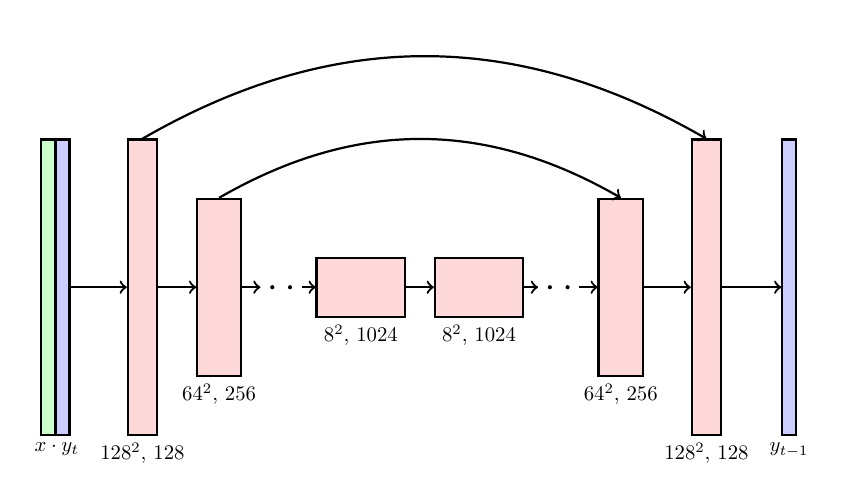
\begin{tikzpicture}[
scale=0.75, every node/.style={scale=0.75}, dot/.style = {circle, fill, minimum size=#1, inner sep=0pt, outer sep=0pt}, dot/.default = 2pt]

\tikzstyle{layer} = [rectangle, thick, minimum width=4cm, minimum height=0.5cm, align=center, draw=black]
\tikzstyle{arrow} = [thick,->]

\node[fill=green!20] (input_high_res1) at (-1.7,0) [layer,thick,minimum width=0.1cm,minimum height=5cm] {};
\node[label=below:{${\bm{x}} \cdot {\bm{y}}_t$}, text width=0.0cm, minimum height=5cm] (temp) at (-1.55,0)  {};
\node[fill=blue!20] (input_low_res1) at (-1.45,0) [layer,thick,minimum width=0.1cm,minimum height=5cm] {};
\node[fill=red!15, label=below:{$128^2$, 128}] (first_res_d) at (-0.1,0) [layer,thick,minimum width=0.5cm,minimum height=5cm] {};
\draw[arrow] (input_low_res1.east) -- (first_res_d.west); 
\node[fill=red!15, label=below:{$64^2$, 256}] (second_res_d) at (1.2,0) [layer,thick,minimum width=0.75cm,minimum height=3cm] {};
\draw[arrow] (first_res_d.east) -- (second_res_d.west); 
\draw[arrow] (second_res_d.east) -- (1.9,0); 
\node[dot] at (2.1,0) {};
\node[dot] at (2.4,0) {};
\node[fill=red!15, label=below:{$8^2$, 1024}] (last_res_d) at (3.6,0) [layer,thick,minimum width=1.5cm,minimum height=1cm] {};
\draw[arrow] (2.6,0) -- (last_res_d.west); 
\node[fill=red!15, label=below:{$8^2$, 1024}] (first_res_u) at (5.6,0) [layer,thick,minimum width=1.5cm,minimum height=1cm] {};
\draw[arrow] (last_res_d.east) -- (first_res_u.west); 

\node[dot] at (6.8,0) {};
\node[dot] at (7.1,0) {};
\draw[arrow] (first_res_u.east) -- (6.6, 0);

\node[fill=red!15,label=below:{$64^2$, 256}] (second_res_u) at (8.0,0) [layer,thick,minimum width=0.75cm,minimum height=3cm] {};
\draw[arrow] (7.3,0) -- (second_res_u.west);
\node[fill=red!15,label=below:{$128^2$, 128}] (last_res_u) at (9.45,0) [layer,thick,minimum width=0.5cm,minimum height=5cm] {};
\draw[arrow] (second_res_u.east) -- (last_res_u.west);
\node[label=below:${\bm{y}}_{t-1}$,fill=blue!20] (output) at (10.85,0) [layer,thick,minimum width=0.15cm,minimum height=5cm] {};
\draw[arrow] (last_res_u.east) -- (output.west);

\draw[arrow] (first_res_d.north) to [out=30,in=150] (last_res_u.north);
\draw[arrow] (second_res_d.north) to [out=30,in=150] (second_res_u.north);

\end{tikzpicture}

The network architecture is based on the 256$\times$256 class-conditional U-Net model of \cite{dhariwal2021diffusion}. The two main differences between our architecture and theirs are (i) absence of class-conditioning, and (ii) additional conditioning of the source image via concatenation, following \cite{saharia2021image}.

\section{Evaluation protocol}

Evaluating image-to-image translation models is challenging.

Prior work on colorization \citep{zhang2016colorful, guadarrama2017pixcolor, coltran}  relied on FID scores and human evaluation for model comparison. Tasks like inpainting \citep{yu2019free, yu2018generative} and uncropping \citep{teterwak2019boundless, wang2019wide} have often heavily relied on qualitative evaluation. For other tasks, like JPEG restoration \citep{dong2015compression,liu2018multi,galteri2019deep}, it has been common to use reference-based pixel-level similarity scores such as PSNR and SSIM. It is also notable that many tasks lack a standardized dataset for evaluation, e.g. different test sets with method-specific splits are used for evaluation.

We propose a unified evaluation protocol for inpainting, uncropping, and JPEG restoration on ImageNet \citep{deng2009imagenet}, due to its scale, diversity, and public availability. For inpainting and uncropping, existing work has relied on Places2 dataset \citep{zhou2017places} for evaluation. Hence, we also use a standard evaluation setup on Places2 for these tasks. Specifically, we advocate the use of ImageNet ctest10k split proposed by \cite{larsson2016learning} as a standard subset for benchmarking of all image-to-image translation tasks on ImageNet. We also introduce a similar category-balanced 10,950 image subset of Places2 validation set called \textit{places10k}. We further advocate the use of automated metrics that capture both image quality and diversity, in addition to controlled human evaluation. We avoid pixel-level metrics like PSNR and SSIM as they  are not reliable measures of sample quality for difficult tasks that require hallucination, like recent super-resolution work, where \citep{ledig2017photo, dahl2017pixel, menon2020pulse} observe that PSNR and SSIM tend to prefer blurry regression outputs, unlike human perception.

We use four automated quantitative measures of sample quality for image-to-image translation: {\bf Inception Score (IS)}~\citep{salimans-iclr-2017}; {\bf Fréchet Inception Distance (FID)}; {\bf Classification Accuracy (CA)} (top-1) of a pre-trained ResNet-50 classifier; and  a simple measure of {\bf Perceptual Distance (PD)}, i.e. Euclidean distance in Inception-v1 feature space (c.f., \cite{DosovitskiyBrox2016}). To facilitate benchmarking on our proposed subsets, we release our model outputs together with other data such as the inpainting masks (see \url{https://bit.ly/eval-pix2pix}).
See Appendix C.5 for more details about our evaluation. For some tasks, we also assess \textbf{sample diversity} through pairwise SSIM and LPIPS scores between multiple model outputs. Sample diversity is challenging and has been a key limitation of many existing GAN-based methods \citep{zhu2017multimodal, yang2019diversity}.

The ultimate evaluation of image-to-image translation models is \textbf{human evaluation}; i.e. whether or not humans can discriminate model outputs from natural images. To this end we use 2-alternative forced choice (2AFC) trials to evaluate the perceptual quality of model outputs against natural images from which we obtained test inputs ({\em c.f.,}~the Colorization Turing Test~\citep{zhang2016colorful}). We summarize the results in terms of the \textbf{fool rate}, the percentage of human raters who select model outputs over natural images when they were asked ``Which image would you guess is from a camera?''. (See Appendix C for details.)

\section{Experiments}

We apply Palette to a suite of challenging image-to-image  tasks:

\begin{enumerate}[topsep=0.1pt, partopsep=0pt, leftmargin=20pt, parsep=0pt, itemsep=0.1pt]
    \item \textbf{Colorization} transforms an input grayscale image to a plausible color image.
    \item \textbf{Inpainting} fills in user-specified masked regions of an image with realistic content. 
    \item \textbf{Uncropping} extends an input image along one or more directions to enlarge the image.
    \item \textbf{JPEG restoration} 

    corrects for JPEG compression artifacts, restoring plausible image detail.
\end{enumerate}

We do so without task-specific hyper-parameter tuning, architecture customization, or any auxiliary loss function. Inputs and outputs for all tasks are represented as  256$\times$256 RGB images. Each task presents its own unique challenges.

Colorization entails a  representation of objects, segmentation and layout, with long-range image dependencies. Inpainting is  challenging with large masks, image diversity and cluttered scenes. Uncropping is widely considered even more challenging than inpainting as there is less surrounding  context to constrain semantically meaningful generation. While the other tasks are linear in nature, JPEG restoration is a non-linear inverse problem; it requires a good local model of natural image statistics to detect and correct compression artifacts. While previous work has studied these problems extensively, it is rare that a model with no task-specific engineering achieves strong performance in all tasks, beating strong task-specific GAN and regression baselines. Palette uses an $L_2$ loss for the denoising objective, unless otherwise specified. (Implementation details can be found in Appendix B.)

\subsection{Colorization}

While prior works \citep{zhang2016colorful, coltran} have adopted LAB or YCbCr color spaces to represent output images for colorization, we use the RGB color space to maintain generality across tasks. Preliminary experiments indicated that Palette is equally effective in YCbCr and RGB spaces. We compare Palette with  Pix2Pix~\citep{isola2017image}, PixColor~\citep{guadarrama2017pixcolor}, and ColTran~\citep{coltran}. Qualitative results are shown in Fig.\, \ref{fig:colorization_comparison}, with quantitative scores in Table \ref{tab:colorization_results}.
Palette establishes a new SoTA, outperforming existing works by a large margin. Further, the performance measures (FID, IS, and CA) indicate that Palette outputs are close to being indistinguishable from the original images that were used to create the test greyscale inputs.

Surprisingly, our $L_2$ Regression baseline also outperforms prior task-specific techniques, highlighting the importance of modern architectures and large-scale training, even for a basic Regression model. On human evaluation, Palette improves upon human raters' fool rate of ColTran by more than 10\%, approaching an ideal fool rate of 50\%.  

\subsection{Inpainting}

We follow \cite{yu2019free} and train inpainting models on free-form generated masks, augmented with simple rectangular masks. To maintain generality of Palette across tasks, in contrast to prior work, we do not pass a binary inpainting mask to the models. Instead, we fill the masked region with standard Gaussian noise, which is compatible with denoising diffusion models. The training loss only considers the masked out pixels, rather than the entire image, to speed up training. We compare Palette with DeepFillv2 \citep{yu2019free}, HiFill \citep{yi2020contextual}, Photoshop's \textit{Content-aware Fill}, and Co-ModGAN \citep{zhao2021large}. While there are other important prior works on image inpainting, such as \citep{liu2018image, liu2020rethinking, zheng2019pluralistic}, we were not able to compare with all of them.

Qualitative and quantiative results are given in Fig.\ \ref{fig:inpainting_comparison} and Table \ref{tab:inpainting_results}. Palette exhibits strong performance across inpainting datasets and mask configurations, outperforming DeepFillv2, HiFill and Co-ModGAN by a large margin. Importantly, like the colorization task above, the FID scores for Palette outputs in the case of  20-30\% free-form masks, are extremely close to FID scores on the original images from which we created the masked test inputs. See Appendix C.2 for more results.

\subsection{Uncropping} 

Recent works \citep{teterwak2019boundless,lin2021infinitygan} have shown impressive visual effects by extending (extrapolating) input images along the right border. We train Palette on uncropping in any one of the four directions, or around the entire image border on all four sides. In all cases, we keep the area of the masked region at 50\% of the image. Like inpainting, we fill the masked region with Gaussian noise, and keep the unmasked region fixed during inference. We compare Palette with  Boundless~\citep{teterwak2019boundless} and InfinityGAN~\citep{lin2021infinitygan}. While other uncropping methods exist (e.g., \citep{guo2020spiral, wang2019wide}), we only compare with  two representative methods. From the results in Fig.\ \ref{fig:extrapolation_comparison} and Table \ref{tab:extrapolation_results}, one can see that Palette outperforms baselines on  ImageNet and Places2 by a large margin.

On human evaluation, Palette has a 40\% fool rate, compared to 25\% and 15\% for Boundless and InfinityGAN (see Fig. C.2 in the Appendix for details).

We further assess the robustness of Palette by generating panoramas through repeated application of left and right uncropping (see Fig.\ \ref{fig:panormauncrop}).
We observe that Palette is surprisingly robust, generating realistic and coherent outputs even after 8 repeated applications of uncrop. We also generate zoom-out sequences by repeated uncropping around the entire border of the image with similarly appealing results (\url{https://diffusion-palette.github.io/}).

\subsection{JPEG restoration}

Finally, we evaluate Palette on the task of removing JPEG compression artifacts, a long standing image restoration problem \citep{dong2015compression, galteri2019deep, liu2018multi}. Like prior work \citep{ehrlich2020quantization, liu2018multi}, we train Palette on inputs compressed with various quality factors (QF). While prior work has typically limited itself to a Quality Factor $\geq$ 10, we increase the difficulty of the task and train on Quality Factors as low as 5, producing severe compression artifacts. Table \ref{tab:compression_results} summarizes the ImageNet results, with Palette exhibiting strong performance across all quality factors, outperforming the regression baseline. As expected, the performance gap between Palette and the  regression baseline widens with decreasing quality factor. Figure \ref{fig:jpeg_comparison} shows the qualitative comparison between Palette and our Regression baseline at a quality factor of 5. It is easy to see that the regression model produces blurry outputs, while Palette produces sharper images. 

\subsection{Self-attention in diffusion model architectures}

Self-attention layers \citep{vaswani-nips-2017} have been an important component in recent U-Net architectures for diffusion models \citep{ho2020denoising, dhariwal2021diffusion}. While self-attention layers provide a direct form of global dependency, they prevent generalization to unseen image resolutions. Generalization to new resolutions at test time is convenient for many image-to-image  tasks, and therefore previous works have  relied primarily on fully convolutional architectures \citep{yu2019free, galteri2019deep}.

We analyze the impact of these self-attention layers on sample quality for inpainting, one of the more difficult image-to-image translation tasks. In order to enable input resolution generalization for Palette, we explore replacing global self-attention layers with different alternatives each of which represents a trade-off between large context dependency, and resolution robustness. In particular, we experiment with the following four configurations:

\begin{enumerate}[topsep=0.21pt, partopsep=0pt, leftmargin=13pt, parsep=0pt, itemsep=0.1pt]
    \item \textbf{Global Self-Attention}: Baseline configuration with global self-attention layers at 32$\times$32, 16$\times$16 and 8$\times$8 resolutions. 
    \item \textbf{Local Self-Attention}: Local self-attention layers \citep{vaswani2021scaling} at 32$\times$32, 16$\times$16 and 8$\times$8 resolutions, at which feature maps are divided into 4 non-overlapping query blocks.
    \item \textbf{More ResNet Blocks w/o Self-Attention}: 2 $\times$ residual blocks at 32$\times$32, 16$\times$16 and 8$\times$8 resolutions allowing deeper convolutions to increase receptive field sizes.
    \item \textbf{Dilated Convolutions w/o Self-Attention}: Similar to 3. ResNet blocks at 32$\times$32, 16$\times$16 and 8$\times$8 resolutions with increasing dilation rates \citep{chen2017rethinking} allowing exponentially increasing receptive fields.
\end{enumerate}

We train models for 500K steps, with a batch size of 512. Table \ref{tab:architecture ablations} reports the performance of different configurations for inpainting. Global self-attention offers  better performance than fully-convolutional alternatives (even with $15\%$ more parameters), re-affirming the importance of self-attention layers for such tasks.  Surprisingly, local self-attention performs worse than fully-convolutional alternatives. Sampling speed is slower than GAN models. There is a large overhead for loading models and the initial  jit compilation, but for 1000 test images, Palette requires 0.8 sec./image on a TPUv4.

\subsection{Sample diversity}

We next analyze sample diversity of Palette on two tasks, colorization and inpainting. Specifically, we analyze the impact of the changing the diffusion loss function $L_{simple}$ \citep{ho2020denoising}, and compare $L_1$ vs. $L_2$ on sample diversity. While existing conditional diffusion models, SR3 \citep{saharia2021image} and WaveGrad \citep{chen-iclr-2021}, have found $L_{1}$ norm to perform better than the conventional $L_{2}$ loss, there has not been a detailed comparison of the two. To quantitatively compare sample diversity, we use multi-scale SSIM \cite{guadarrama2017pixcolor} and the  LPIPS diversity score \cite{zhu2017multimodal}. Given multiple generated outputs for each input image, we compute pairwise multi-scale SSIM between the first output sample and the remaining samples. We do this for multiple input images, and then plot the histogram of SSIM values (see Fig.\ \ref{fig:diversity_ssim}). 
Following  \cite{zhu2017multimodal}, we also compute LPIPS scores between consecutive pairs of model outputs for a given input image, and then average  across all outputs and input images. Lower SSIM and higher LPIPS scores imply more sample diversity. The results in Table \ref{tab:diversity_table} thus clearly show that models trained with the $L_2$ loss have greater sample diversity than those trained with the $L_1$ loss.

Interestingly,  Table \ref{tab:diversity_table} also indicates that $L_1$ and $L_2$ models yield similar FID scores (i.e.,  comparable perceptual quality), but that $L_1$ has somewhat lower  Perceptual Distance scores than $L_2$. One can speculate that $L_1$ models may drop more modes than $L_2$ models, thereby increasing the likelihood that  a single sample from an $L_1$ model is from the mode containing the corresponding original image, and hence a smaller Perceptual Distance.

Some existing GAN-based models explicitly encourage diversity;  \citep{zhu2017multimodal, yang2019diversity} propose methods for improving diversity of conditional GANs, and \citep{zhao2020uctgan, han2019finet} explore diverse sample generation for image inpainting. We leave comparison of sample diversity between Palette and other such GAN based techniques to future work.

\subsection{Multi-task learning}

Multi-task training is a natural approach to learning a single model for multiple image-to-image tasks, i.e., blind image enhancement.

Another is to adapt an unconditional model to conditional tasks with imputation. For example, \cite{song-iclr-2021} do this for inpainting; in each step of iterative refinement, they denoise the noisy image from the previous step, and then simply replace any pixels in the estimated image ${\bm{y}}$ with pixels from the observed image regions, then adding noise and proceeding to the next denoising iteration. Figure \ref{fig:uncond_inpaint_main_paper} compares this method  with a multi-task Palette model trained on all four tasks, and a Palette model trained solely on inpainting.  All models use the same architecture, training data and number of training steps. The results in Fig.\ \ref{fig:uncond_inpaint_main_paper} are typical; the re-purposed unconditional model does not perform well, in part because it is hard to learn a good unconditional model on diverse datasets like ImageNet, and also because, during iterative refinement, noise is added to all pixels, including the observed pixels.  By contrast, Palette is condition directly on noiseless observations for all steps.

To explore the potential for multi-task models in greater depth, Table \ref{tab:multitask_results}
provides a quantitative comparison between a single generalist Palette model trained simultaneously on JPEG restoration, inpainting, and colorization. It indicates that multi-task generalist Palette outperforms the task-specific JPEG restoration specialist model, but slightly lags behind task-specific Palette models on inpainting and colorization. The multi-task and task-specific Palette models had the same number of training steps; we expect multi-task  performance to improve with more training.

\section{Conclusion}

We present Palette, a simple, general framework for image-to-image translation.

Palette achieves strong results on four challenging image-to-image translation tasks (colorization, inpainting, uncropping, and JPEG restoration), outperforming strong GAN and regression baselines. Unlike many GAN models, Palette produces diverse and high fidelity outputs. This is accomplished without task-specific customization nor optimization instability. We also present a multi-task Palette model, that performs just as well or better over their task-specific counterparts. Further exploration and investigation of multi-task diffusion models is an exciting avenue for future work. 

This paper shows some of the potential of image-to-image diffusion models, but we look forward to seeing new applications.

\subsection*{Acknowledgements}
We thank John Shlens, Rif A. Saurous, Douglas Eck and the entire Google Brain team for helpful discussions and valuable feedback. We thank Lala Li for help preparing the codebase for public release, and  Erica Moreira for help with compute resources. We also thank Austin Tarango and Philip Parham for help with the approvals for releasing the paper, codebase and checkpoints. 

\end{document}
